\begin{figure}

  \setlength{\unitlength}{\textwidth}
%  \fbox{
  \begin{picture}(1,0.58)(0,0.35)
    % % % 90
    \put(0.03,0.76){\includegraphics[width=0.35\unitlength]{../FnP/gnuplot/power_time_history_015.eps}}
    \put(0.03,.58){\includegraphics[width=0.35\unitlength]{../FnP/gnuplot/f_y_history_015.eps}}
    \put(0.03,0.4){\includegraphics[width=0.35\unitlength]{../FnP/gnuplot/theta_time_history_015.eps}}
    
    % % 165
    \put(0.36,0.76){\includegraphics[width=0.35\unitlength]{../FnP/gnuplot/power_time_history_54.eps}}
    \put(0.36,.58){\includegraphics[width=0.35\unitlength]{../FnP/gnuplot/f_y_history_54.eps}}
    \put(0.36,0.4){\includegraphics[width=0.35\unitlength]{../FnP/gnuplot/theta_time_history_54.eps}}
    
    \put(0.68,0.76){\includegraphics[width=0.35\unitlength]{../FnP/gnuplot/power_time_history_08.eps}}
    \put(0.68,.58){\includegraphics[width=0.35\unitlength]{../FnP/gnuplot/f_y_history_08.eps}}
    \put(0.68,0.4){\includegraphics[width=0.35\unitlength]{../FnP/gnuplot/theta_time_history_08.eps}}
    
    \put(0.55,0.36){$\displaystyle{\frac{tU}{D}}$}
    \put(0.2,0.36){$\displaystyle{\frac{tU}{D}}$}
    \put(0.85,0.36){$\displaystyle{\frac{tU}{D}}$}
    
    \put(0.0,0.87){$\frac{P}{\rho \mathcal{A}U^3}$}
    \put(0.01,0.66){$F_y$}
    \put(0.01,0.49){$\theta$}
    
    \put(0.08,0.76){(a)}
    \put(0.08,0.58){(d)}
    \put(0.08,0.38){(g)}
    
    \put(0.4,0.76){(b)}
    \put(0.4,0.58){(e)}
    \put(0.4,0.38){(h)}
    
    \put(0.72,0.76){(c)}
    \put(0.72,0.58){(f)}
    \put(0.72,0.38){(i)}
  \end{picture}
%}
  \caption{Time histories of $P_t$, $P_d$, $F_y$ and $\theta$ at $\massdamp=0.15$, $0.54$ and $0.8$ from the QSS model. Data was obtained at $m^*=20$, $\massstiff=10$ and \reynoldsnumber=200. The time histories of $P_t$ ( \solidrule[4mm]\hspace{1mm}) and $P_d$ (\protect\dashedrule) are presented for: (a) $\massdamp= 0.15$; (b) $\massdamp= 0.54$; (c) $\massdamp= 0.8$. Time histories of the instantaneous force $F_y$ for: (d) $\massdamp= 0.15$; (e) $\massdamp= 0.54$; (f) $\massdamp= 0.8$. Time histories of the instantaneous angle $\theta$ for: (g) $\massdamp= 0.15$; (h) $\massdamp= 0.55$; (i) $\massdamp= 0.8$.}
  \label{fig:power_time_histories}
\end{figure}




